\section{User Functionality Abstract}

\subsection{Components}

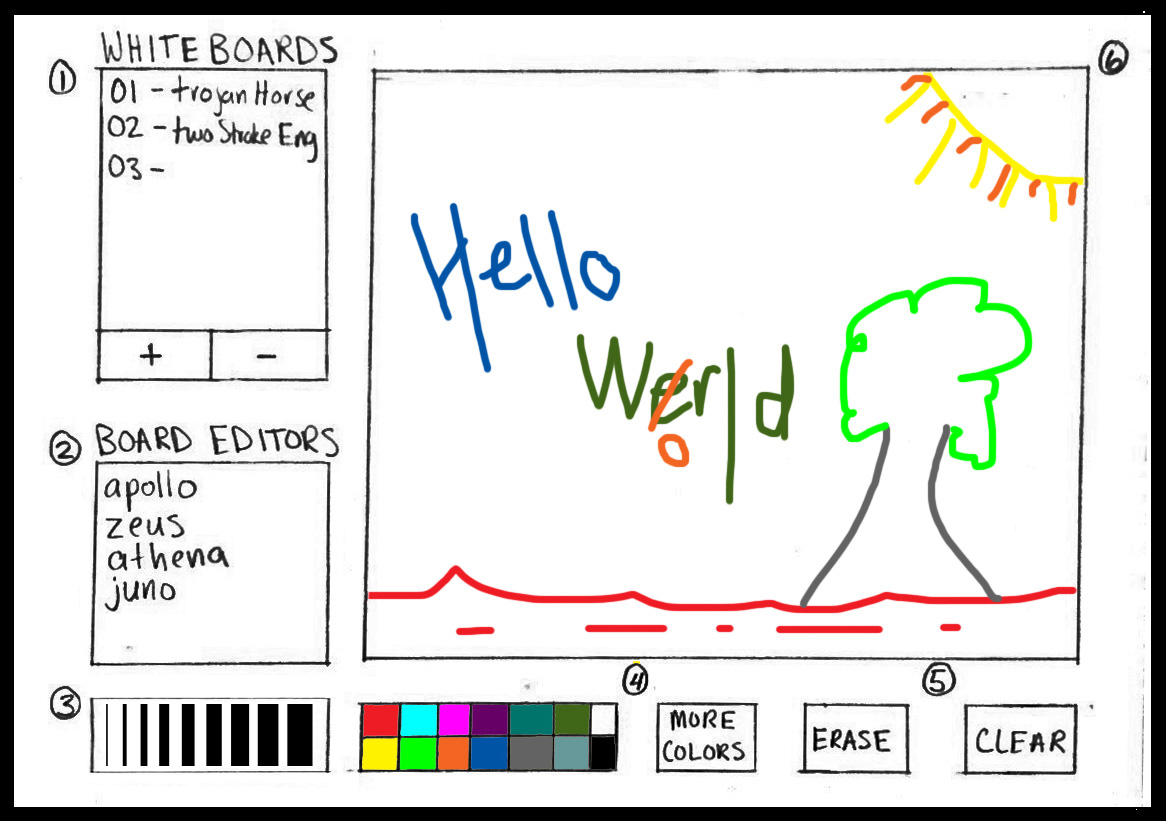
\includegraphics[keepaspectratio=1,width=6in]{img/gui-sketch.jpg}

\subsubsection{Selector}

The board selector in the left pane includes a list of all current whiteboards and appears the same for all users. Each line represents an individual board, which are numbered sequentially and named by the user. Upon clicking the "+" button, the user will be prompted to name the new board. When the board has been created on the server, it will be appended to the list for each user. Selecting a board in the list will download the board from the server, overwrite the local copy if one exists, and display the board in the canvas window. 

\subsubsection{Board Editors}

Displays a list of users, including the viewer, who are currently modifying the selected board. This list will be updated as users enter and exit the board.

\subsubsection{Thickness Selector}

This tool allows the user to select a brush/eraser thickness for drawing on the whiteboard.

\subsubsection{Color Selector}

The main color palette displays a grid of colors from which the user can choose to paint with. The color currently in use will be highlighted. Clicking the "more colors" button will open Swing's built-in color chooser, which will offer a larger selection of colors.

\subsubsection{Erasing Tools}

The erase button will allow the user to toggle between erasing and painting. "Erasing" will be defined as drawing with a white selection. Erasing will happen in the same order as drawing, so whichever request reaches the server first will erase all that has been drawn under it. Toggling back to painting will restore the user's previous color choice.

\subsubsection{Whiteboard Window}

Displays the currently selected whiteboard, including all of its drawn strokes and erasures. The whiteboard be real-time interactive to allow users to collaborate simultaneously. Edits will be made in the order that modifications reach the server. In other words, a stroke logged on the server at a specific instant will be drawn over any strokes drawn before that instant.

\subsection{Behavior}

\paragraph{Erasing}

Because the default canvas color is white, erasing will function the same as drawing with the color white selected.  The thickness functionality that is present during normal drawing will continue to work with erasing. The Erase button on the client GUI will function as a toggle. Clicking the button once will switch to erasing mode, which essentially is simply switching the client's selected color to white. At this time, the user's previously selected color will be stored for future use. Clicking the button a second time will return the user's selected color to what is was before the user entered erasing mode.

\paragraph{Editing a Deleted Board}

Clients should not be allowed to edit a board that has been deleted by another user. To prevent this, users who are working on a board when it is marked for deletion by another user will be presented with a message box, stating that their board has been deleted.  The deleted board then becomes unselected by any client GUIs who had the board selected at the time of deletion, forcing users to select a different whiteboard to work on. Simultaneously, the board will be removed from the master list of whiteboards available, so that no users in the future may accidentally select the deleted board.